%!TEX root = ../TTK4900-MHT.tex

\chapter{Theoretical Background}\label{chapter:theoretical_background}
\section{Radar}
\subsection{Overview}
\gls{radar_acr} is a detection technology that uses radio waves to observe stationary and moving objects. A transmitter sends out radio waves and a receiver is waiting for reflected echo's from objects, the time the echo is delayed determines the distance to the object. The transmitter and receiver will in many situations be in the same location as the transmitter, and can be both stationary and mobile. Depending on frequency, a radar can observe solid objects like air-crafts, ships, terrain, people, road vehicles and weather formations.

\subsection{History}
The fist implementation of an instrument that were able to detect the presence of distance metallic objects by radio waves was done by Christian Hülsmeyer in 1904. His invention did not measure the distance to objects, but whether there was an object in the direction of the instrument. The radar as we know it today was introduced in the mid to late 1930's, with world war two triggering a research to improve the still immature technology to be used in military applications. After the war, the technology matured and where put in use in several civil applications, where air traffic control, maritime safety and weather monitoring is the most common.

\subsection{Principles}
The electromagnetic waves that a radar emits travels at the speed of light in air and vacuum. It reflects back when there is a change in the density of the medium it is travelling through, which is what happens when radio waves hit targets. Electrically conductive materials tends to be good reflectors, since they have a very different atomic density than air. On the other hand, materials with poor conductivity, and also some magnetic materials, then to absorb radio waves good. Like light, there is many ways an incoming radio wave can be reflected, primarily dependent on the geometry of the target. A corner with angles less than 180\degsym{} will reflect the incoming radio waves directly back to the sender, and is a good thing on targets that want to be visible on a radar. This principle are the basis for radar reflectors commonly used to boos the radar signature on smaller vessels, see Figure~\ref{fig:corner_reflector}.
\begin{wrapfigure}{R}{0.3\textwidth}
\centering
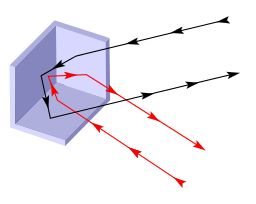
\includegraphics[width=0.25\textwidth]{Corner_reflector}
\caption{Corner reflector}\label{fig:corner_reflector}
\end{wrapfigure}
The opposite is used on targets that try to minimize their radar signature, and is the reason why stealth vessels and aircraft are tiled by flat areas. 
\begin{figure}
\centering
\begin{minipage}{0.3\textwidth}
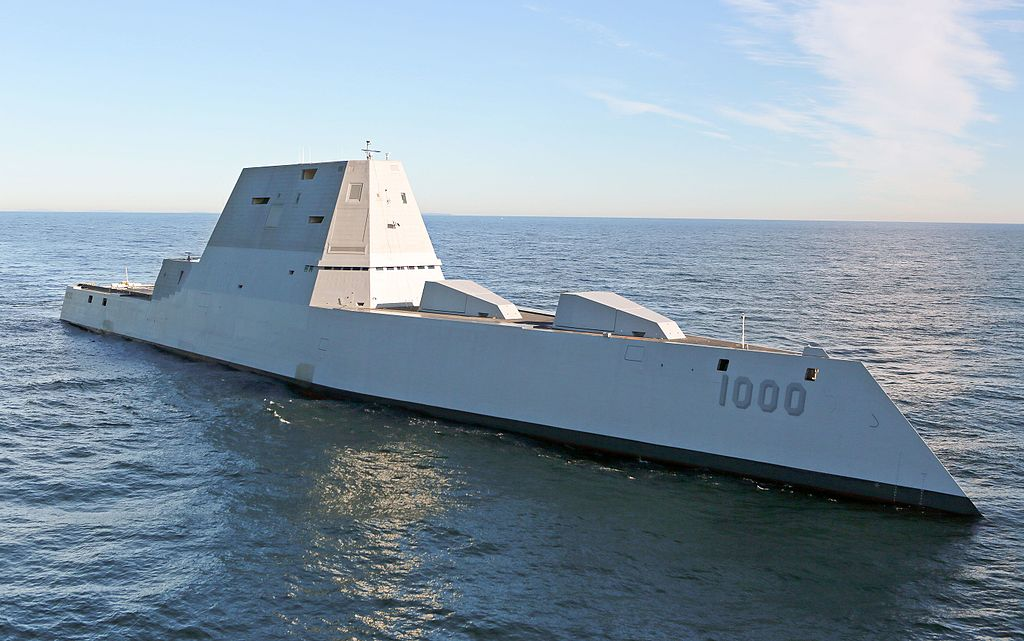
\includegraphics[width=0.9\textwidth]{USS_Zumwalt}
\caption{USS Zumwalt}\label{fig:uss_zumwalt}
\end{minipage}\hfill
\begin{minipage}{0.3\textwidth}
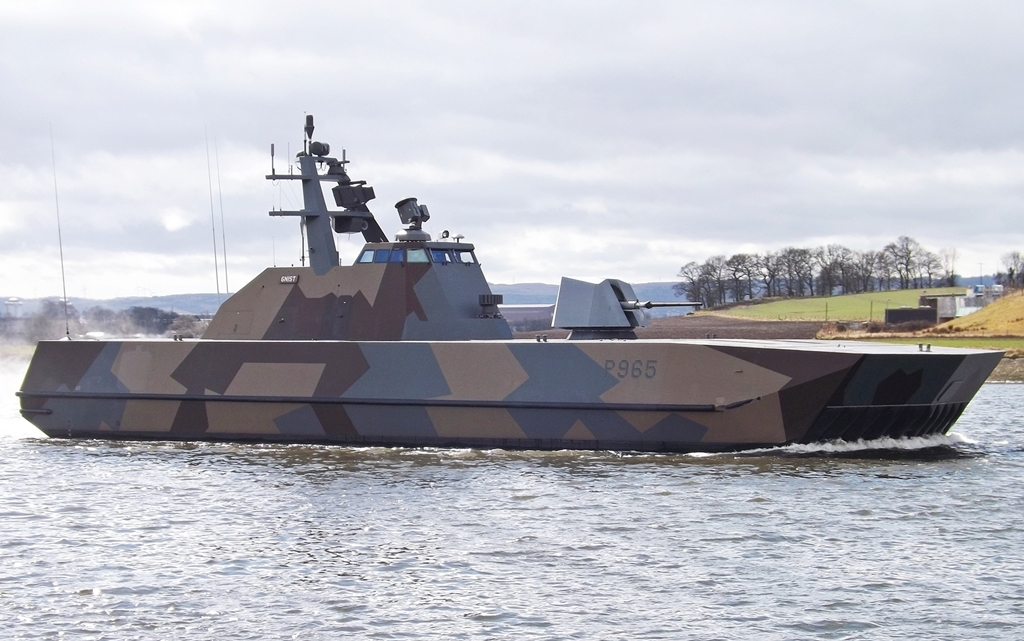
\includegraphics[width=0.9\textwidth]{KNM_Gnist}
\caption{KNM Gnist}\label{fig:knm_gnist}
\end{minipage}\hfill
\begin{minipage}{0.3\textwidth}
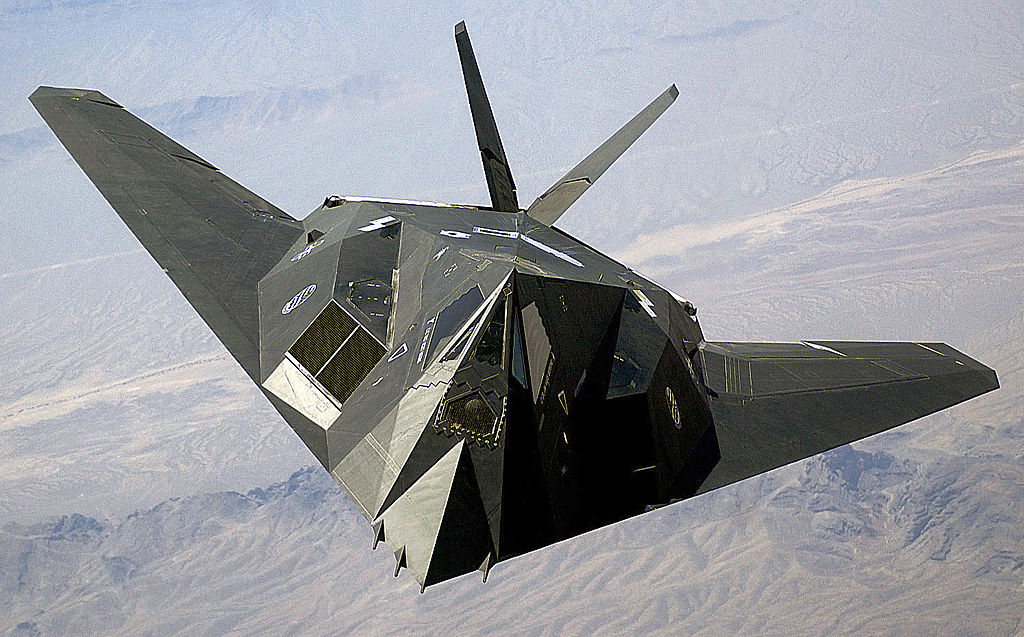
\includegraphics[width=0.9\textwidth]{Figures/F-117_Nighthawk}
\caption{F177 Nighthawk}\label{fig:f177_nighthawk}
\end{minipage}
\end{figure}

\section{AIS}
The \acrfull{ais} is a maritime safety and information system primarily designed for collision avoidance. \gls{ais} works by broadcasting messages on the \gls{vhf} band at irregular intervals with information on the vessels. \gls{ais} transceivers are required on international voyaging vessels over 300 \gls{gross_tonnage}, and on all passenger vessels. \gls{ais} signals are received at bother vessels and shore stations for use in \gls{vts} stations, open tracking databases like \url{www.marinetraffic.com}, fleet-monitoring and search and rescue.

\subsection{History}
\gls{ais} was designed and developed by technical comities in the \gls{imo}. Its objective was to enhance vessels safety and efficiency by increasing their ability to see and identify other vessels. The main motivation for adopting \gls{ais} was its independence of humans in operation, since it automatically identifies other vessels and displays the information on the navigational system on the bridge. It also enables automatic calculation of \gls{cpa} and time until \gls{cpa}, in which the navigation system could alarm the bridge on incoming traffic on dangerous course. This give the navigator on the bridge more and better information for making decisions, but with the caveat that not all vessels have \gls{ais}. In the 2002 IMO SOLAR Agreement it is specified a requirement that vessels over

\subsection{Principles}


\section{Tracking}
\subsection{Overview}
Tracking, in this context, is to follow stationary and moving targets that are observed by a system without included association data. The problem is to know which measurements belong together over time, often refereed to as the data association problem. 

\subsection{History}
Tracking is a relative new filed of study, originating from the military technology race post 1945, enabled by the development of microprocessors and computers from the 60's. The applications ranged from sonar tracking on both submarines and navy vessels, to air control and missile guidance. This historical background is likely the reason for most published papers using these types of applications as background for testing. In recent years, tracking people and vehicles from visual- and \gls{sar} imagery have also become a topic in the research community~\cite{Carthel2007,Carthel2007a,Coraluppi2000}. There have also been published some research work on usage of tracking for \glspl{asv}~\cite{Wolf2010,Svec2014}, although both are focused on interaction and response to external events.

%Challenge
There are several factors contributing to the challenge of good tracking;\gls{clutter}, lower than unity \gls{Pd}, multiple detections of the same vessel and wakes. \Gls{clutter} is a term for unwanted measurements or noise, which is inherent in every observation system. For a maritime radar, this can be caused by waves, rain, snow, birds or shore echo. A common assumption on clutter is to assume the amount being Poisson \gls{Pd} is a measure of how persistent the target is in the measurements, and will vary much  between different types of targets. 

\subsection{Single-target Tracking}
The simplest approach to tracking is single-target tracking, where it is assumed that there are only one target in the measurement area, and any other measurement is regarded as either extra measurements of the target or false measurements, often referred to as \gls{clutter}.

\subsection{Multitarget tracking}
A subset of tracking is multitarget tracking, where the problem expands to jointly estimate both the number of targets and their trajectories. While a large number of tracking techniques have been developed, the three most used are \gls{jpdaf}, \gls{mht} and \gls{rfs}~\cite{Vo2015}.

\subsection{JPDAF}
\gls{jpdaf} is a multitarget expansion of \gls{pdaf} which is a single-target tracking technique. The essence of them both is consider 

\subsection{RFS}

\subsection{MHT}